\section{Capturas del prototipo Figma}
\label{anexo:figma}

\begin{figure}[H]
    \centering
    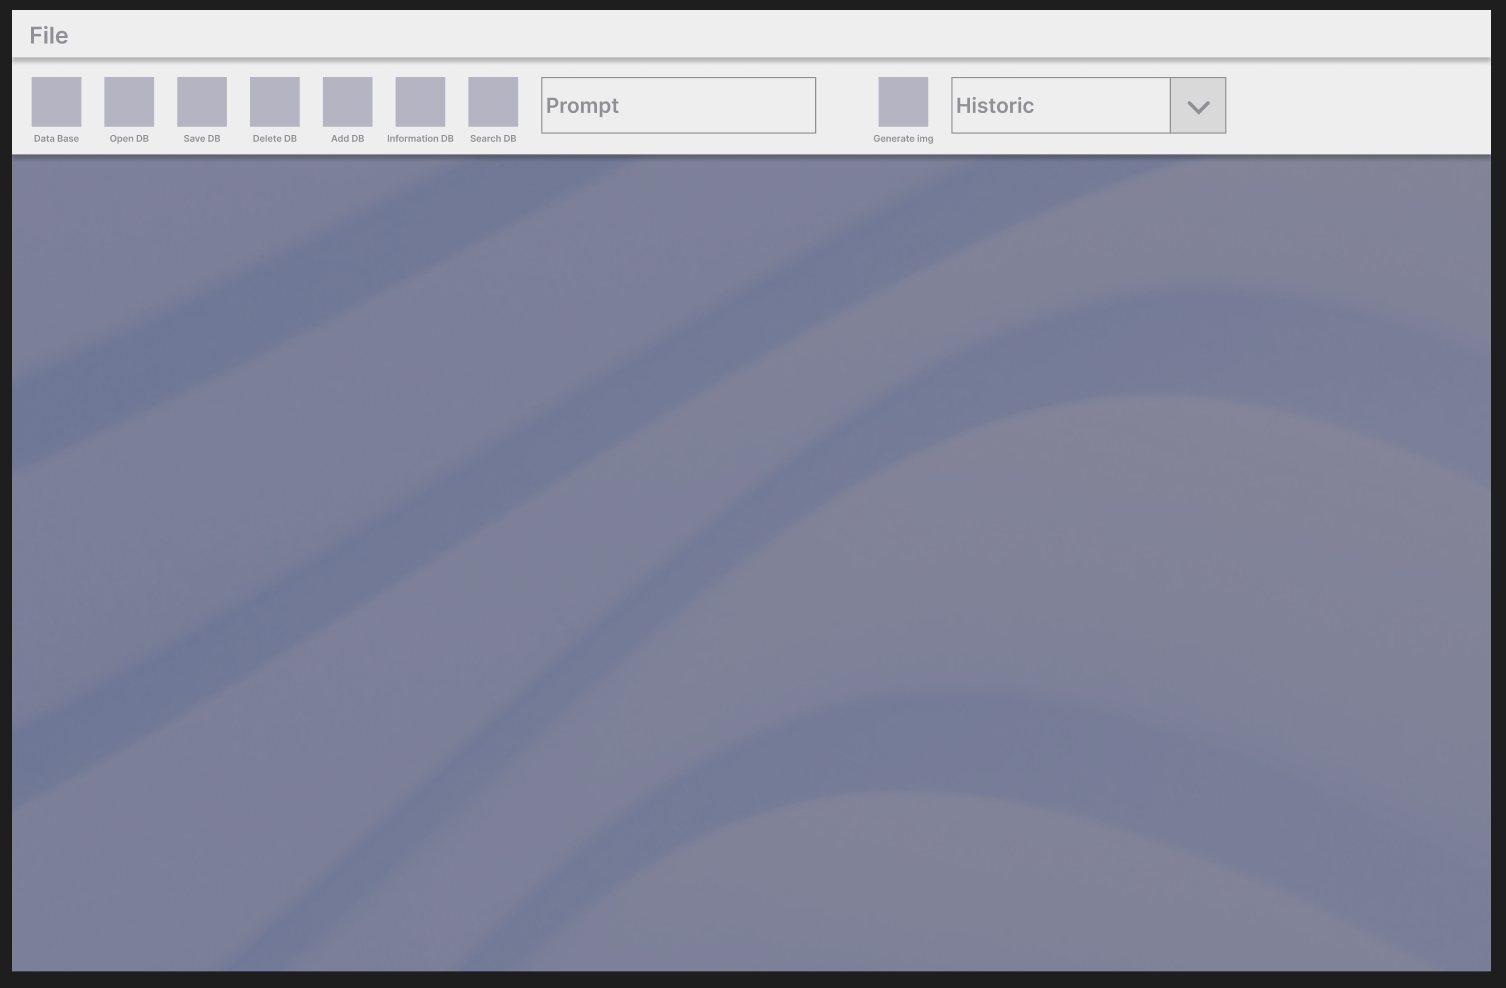
\includegraphics[width=0.85\textwidth]{figma/figma1.png}
    \caption{Pantalla principal del sistema}
\end{figure}

\begin{figure}[H]
    \centering
    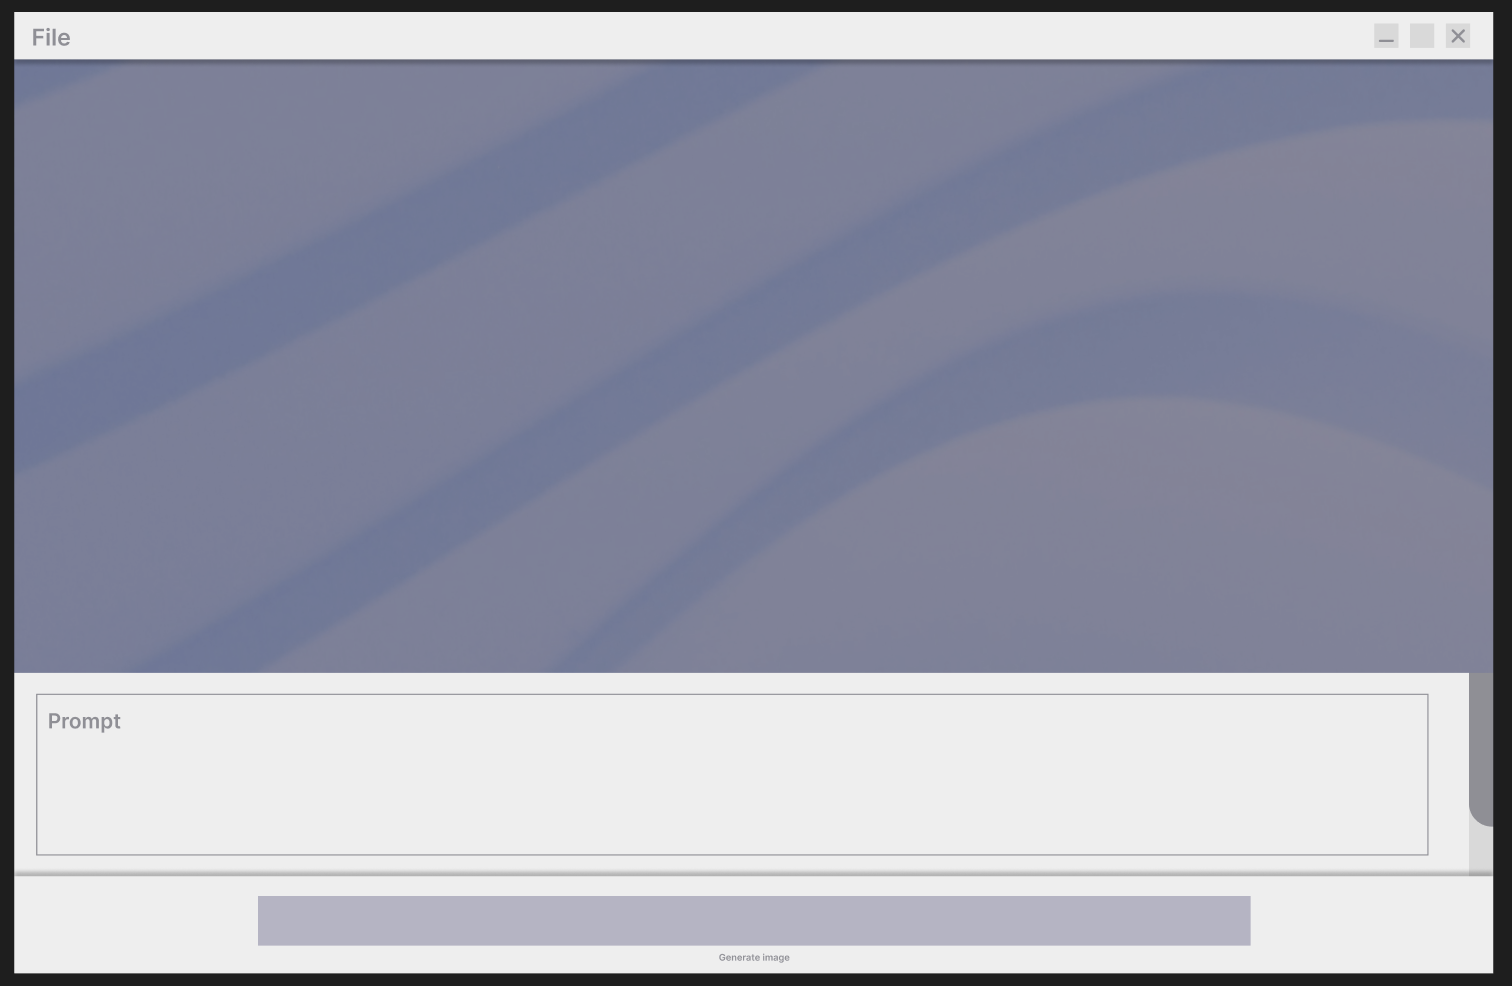
\includegraphics[width=0.85\textwidth]{figma/figma2.png}
    \caption{Ventana emergente de generación de imágenes}
\end{figure}

\begin{figure}[H]
    \centering
    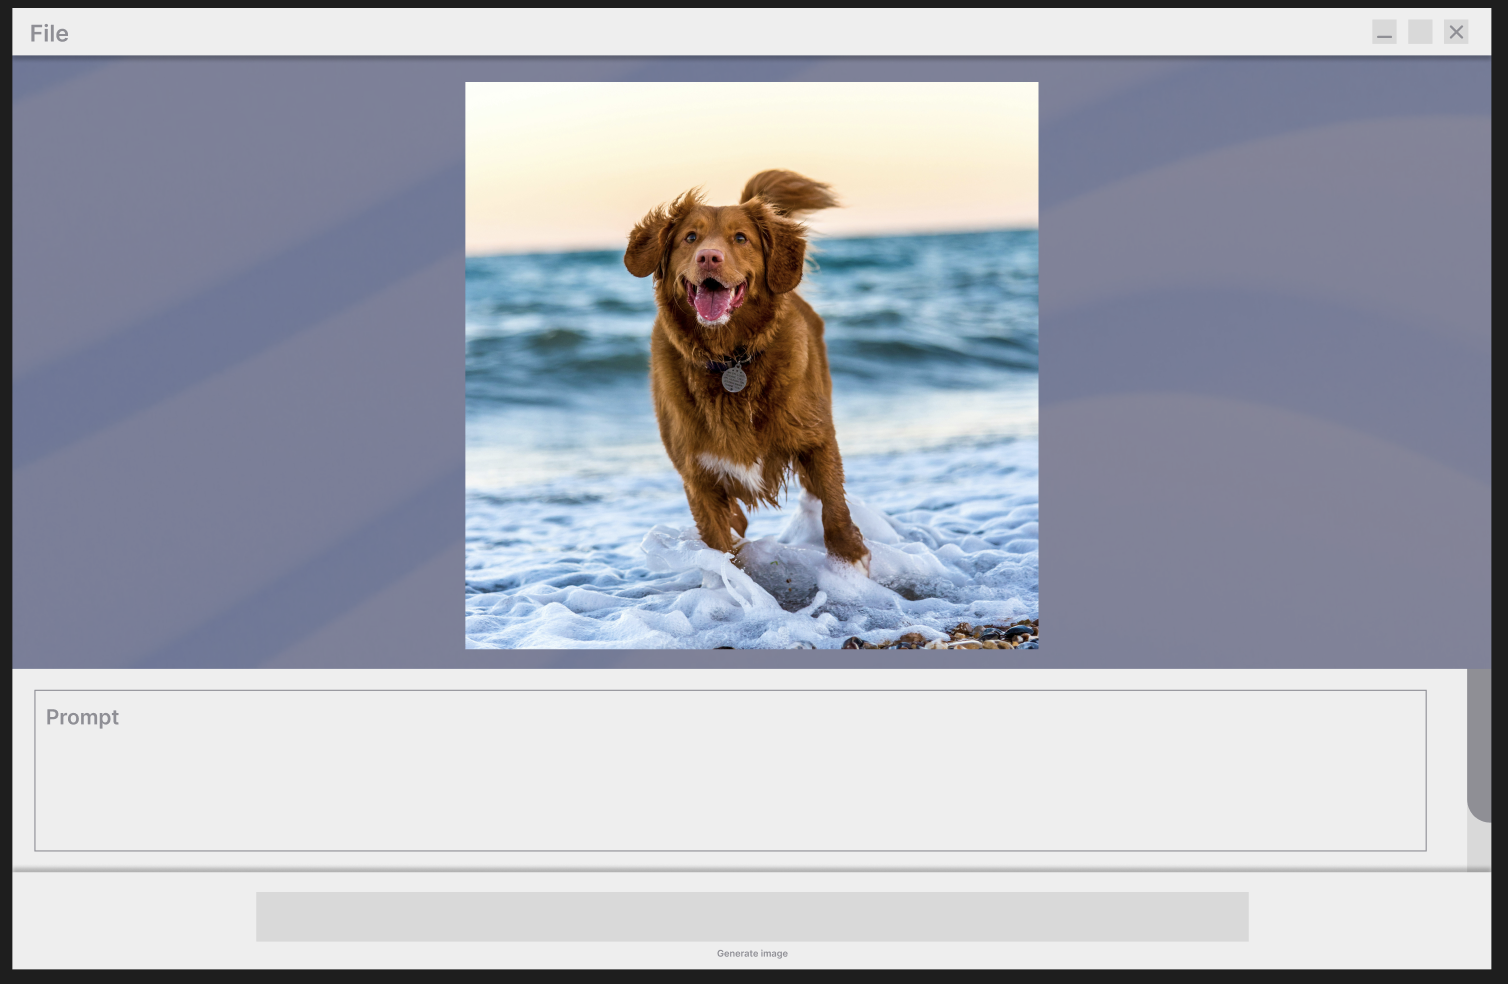
\includegraphics[width=0.85\textwidth]{figma/figma3.png}
    \caption{Imagen generada y visualizada en una ventana}
\end{figure}

\begin{figure}[H]
    \centering
    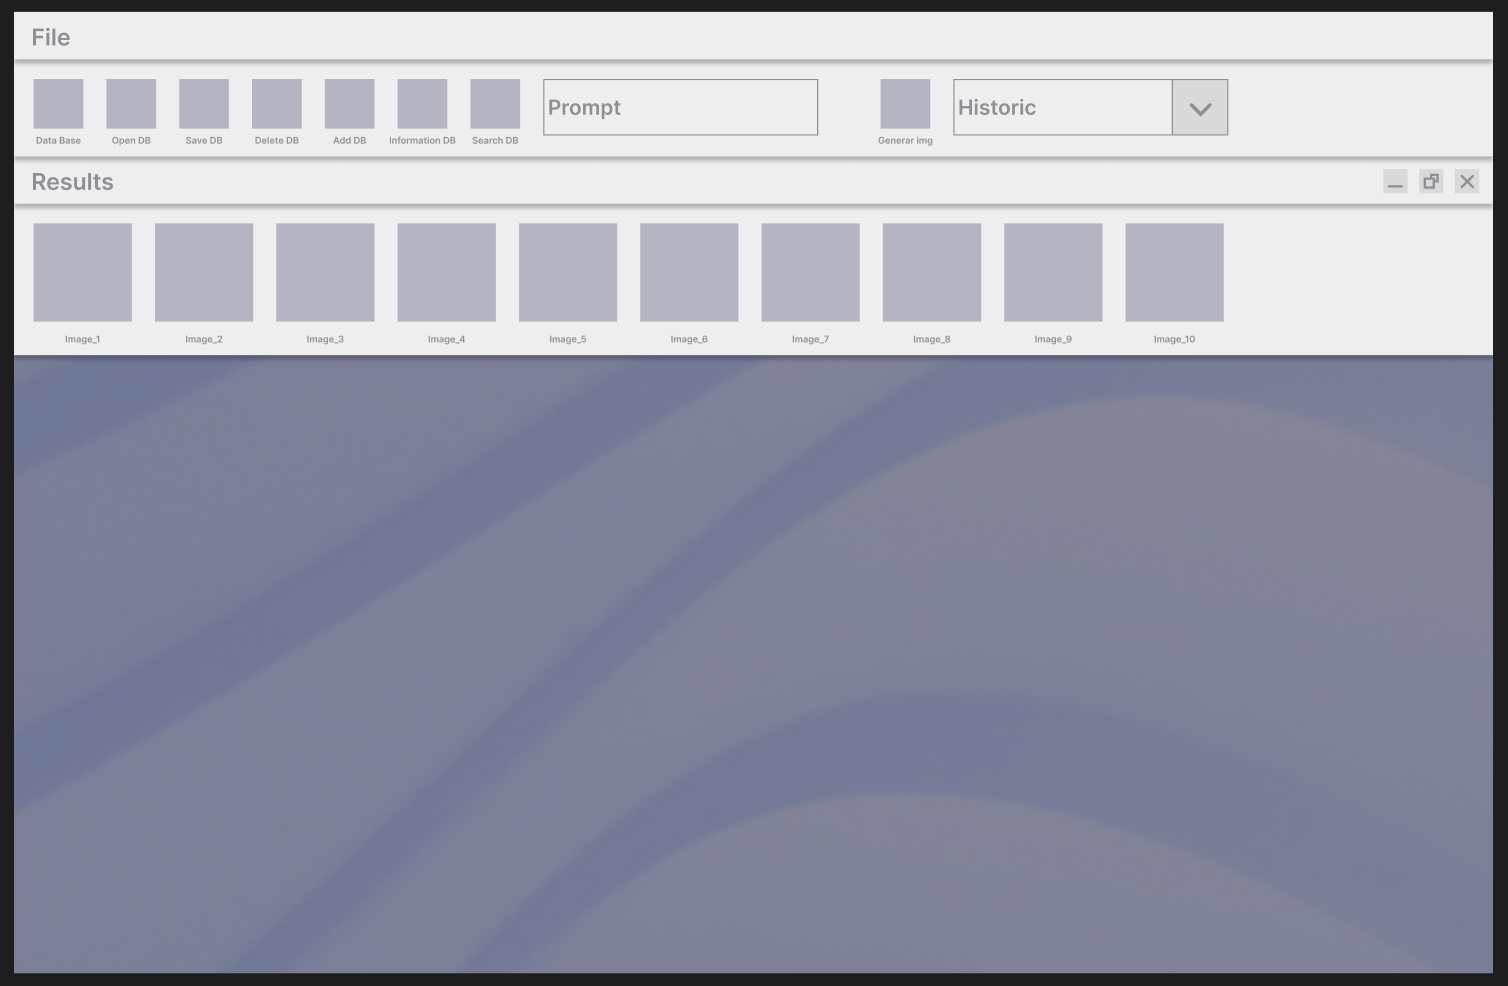
\includegraphics[width=0.85\textwidth]{figma/figma4.png}
    \caption{Galería de resultados con miniaturas}
\end{figure}

\begin{figure}[H]
    \centering
    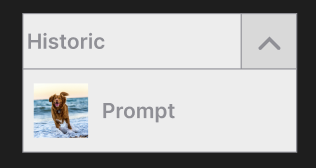
\includegraphics[width=0.5\textwidth]{figma/figma5.png}
    \caption{Histórico de prompts con miniatura}
\end{figure}

\begin{figure}[H]
    \centering
    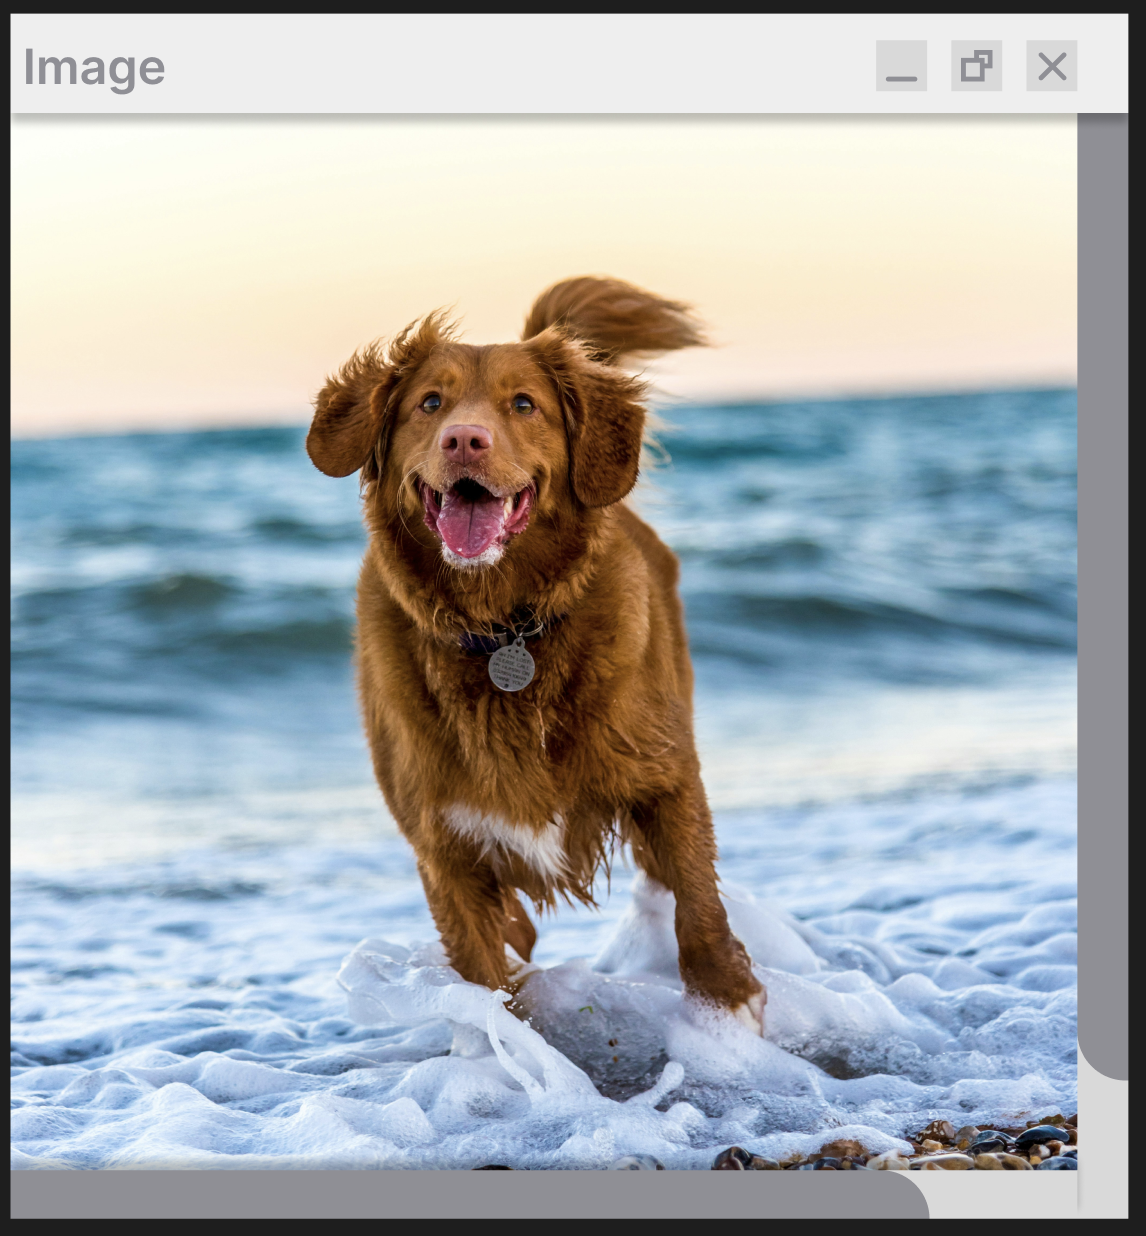
\includegraphics[width=0.5\textwidth]{figma/figma6.png}
    \caption{Resultado de abrir un prompt del histórico}
\end{figure}

\begin{figure}[H]
    \centering
    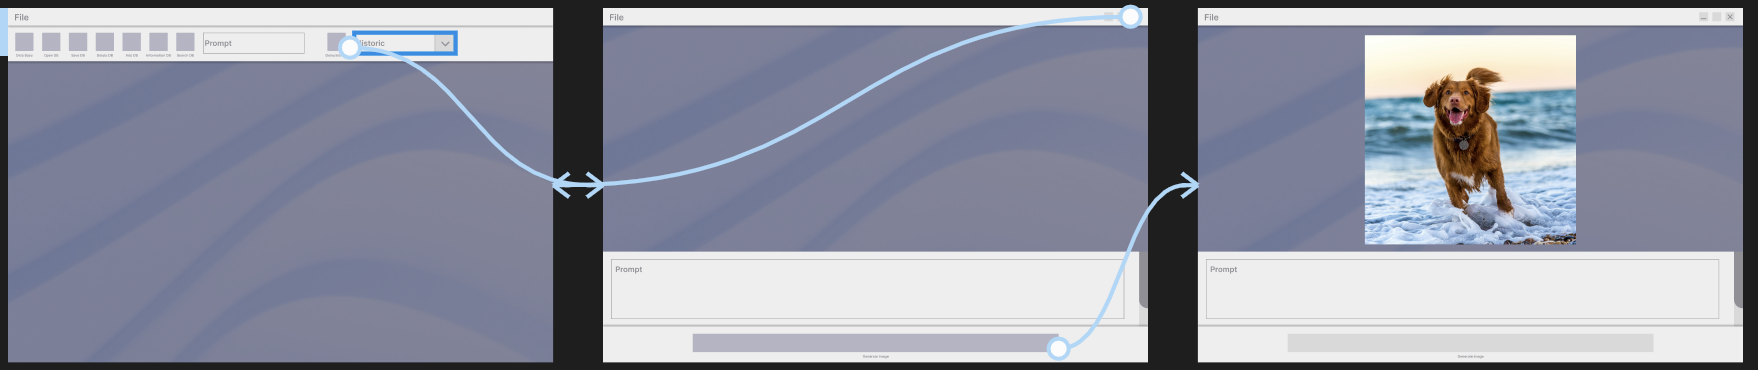
\includegraphics[width=1\textwidth]{figma/figma7.png}
    \caption{Transición desde pantalla principal a ventana de generación}
\end{figure}

\begin{figure}[H]
    \centering
    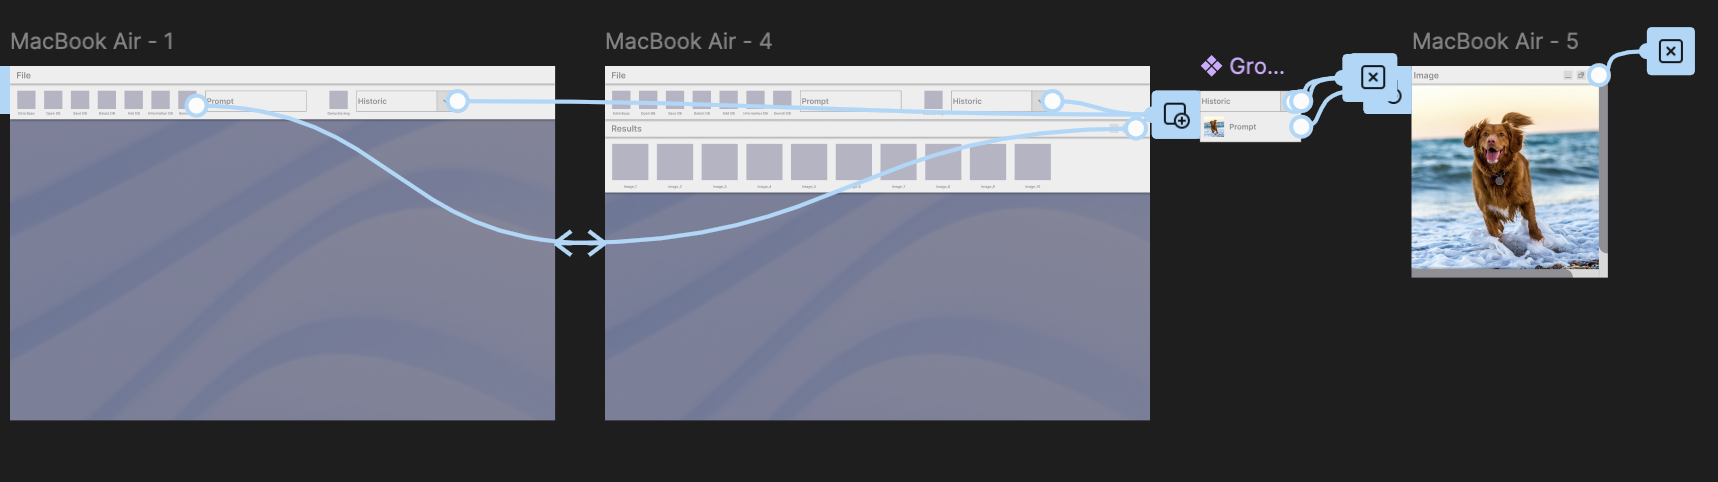
\includegraphics[width=1\textwidth]{figma/figma8.png}
    \caption{Transición desde histórico a ventana de visualización de imagen}
\end{figure}